\documentclass[12pt]{article}

\usepackage{answers}
\usepackage{setspace}
\usepackage{graphicx}
\usepackage{enumitem}
\usepackage{multicol}
\usepackage{mathrsfs}
\usepackage[margin=1in]{geometry} 
\usepackage{amsmath,amsthm,amssymb}
\usepackage[ngerman]{babel}

\newcommand{\N}{\mathbb{N}}
\newcommand{\Z}{\mathbb{Z}}
\newcommand{\C}{\mathbb{C}}
\newcommand{\R}{\mathbb{R}}

\DeclareMathOperator{\sech}{sech}
\DeclareMathOperator{\csch}{csch}

\newenvironment{theorem}[2][Theorem]{\begin{trivlist}
		\item[\hskip \labelsep {\bfseries #1}\hskip \labelsep {\bfseries #2.}]}{\end{trivlist}}
\newenvironment{definition}[2][Definition]{\begin{trivlist}
		\item[\hskip \labelsep {\bfseries #1}\hskip \labelsep {\bfseries #2.}]}{\end{trivlist}}
\newenvironment{proposition}[2][Proposition]{\begin{trivlist}
		\item[\hskip \labelsep {\bfseries #1}\hskip \labelsep {\bfseries #2.}]}{\end{trivlist}}
\newenvironment{lemma}[2][Lemma]{\begin{trivlist}
		\item[\hskip \labelsep {\bfseries #1}\hskip \labelsep {\bfseries #2.}]}{\end{trivlist}}
\newenvironment{exercise}[2][Exercise]{\begin{trivlist}
		\item[\hskip \labelsep {\bfseries #1}\hskip \labelsep {\bfseries #2.}]}{\end{trivlist}}
\newenvironment{solution}[2][Solution]{\begin{trivlist}
		\item[\hskip \labelsep {\bfseries #1}]}{\end{trivlist}}
\newenvironment{problem}[2][Problem]{\begin{trivlist}
		\item[\hskip \labelsep {\bfseries #1}\hskip \labelsep {\bfseries #2.}]}{\end{trivlist}}
\newenvironment{question}[2][Question]{\begin{trivlist}
		\item[\hskip \labelsep {\bfseries #1}\hskip \labelsep {\bfseries #2.}]}{\end{trivlist}}
\newenvironment{corollary}[2][Corollary]{\begin{trivlist}
		\item[\hskip \labelsep {\bfseries #1}\hskip \labelsep {\bfseries #2.}]}{\end{trivlist}}

\begin{document}
	\title{Programmieren mit Neuronalen Netzen}
	\author{Michael Gabler}
	\maketitle
	\tableofcontents
	\newpage

	\section{Grundlagen}
	Neuronales Netzwerk ist Funktion, die auf Eingabedaten angewendet wird.\\
	\textbf{Optimierung} durch Minimierung der Loss-Funktion\\
	\textbf{Loss-Funktion} Maß, wie gut das Netzwerk Vorhersagen trifft. Berechnet sich aus Vorhersage und tatsächlichen Werten (Ground Truth).
	\begin{itemize}
		\item Euklidischer Loss, Mean-Squared-Error: $l_2 = \frac{1}{2N} \sum_i (f_\theta(x_i)-t_i)^2$
		\item Negative-Log-Likelihood, Cross-Entropy: $NLL = -\frac{1}{|D|}\sum_i \log[f_\theta(x_i)|_{t_i}]$
	\end{itemize}
	\textbf{Konfusionsmatrix} welche Klassen werden wie oft mit welcher Klasse verwechselt?\\
	\textbf{Linearisiertes Speichern mehrdimensionaler Objekte}\\
	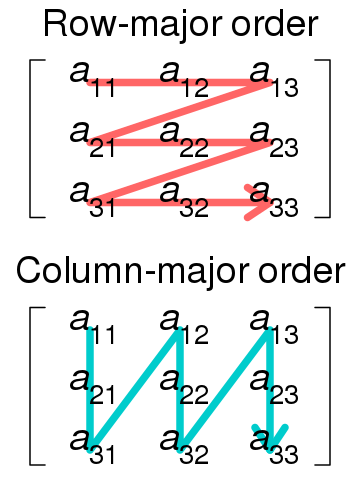
\includegraphics[width=0.25\linewidth]{figures/row-column-major.png}\\

	
	\subsection{Training}
	Daten werden aufgeteilt in Train/Validierung/Test (z.B. 60/20/20)\\
	\textbf{Datenaugmentierung} Generieren zusätzlicher Daten (z.B. bei Bildern) durch Spiegelung, Rotation, Skalierung, Anpassung Helligkeit und Farbe, etc.\\
	\textbf{Epoche} Verarbeitung aller Trainingsdaten\\
	\textbf{Iteration} Verarbeitung eines Batches\\
	\textbf{Batch} Mehrere Trainingsbeispiele werden gerechnet bevor Gewichte einmal geupdated werden (z.B. 10 Beispiele pro Batch)\\
	\textbf{Learning Rate} Faktor $\eta$, wie stark das Netzwerk durch die Deltas verändert werden soll (d.h. wie schnell es lernt bzw. seine Meinung ändert). Wird beim Update der Gewichte verwendet.
	\textbf{Evaluation auf Validierungsdaten} zur Anpassung der Hyperparameter (Learning-Rate, Netzstruktur, ...)\\
	\textbf{Evaluation auf Testdaten} einmalig, um Genauigkeit des trainierten Netzes zu ermitteln
	\textbf{Forward-Pass} Berechnen des Outputs des Netzwerkes für bestimmte Eingabedaten (z.B. ein Batch)\\
	\textbf{Backward-Pass} Bilden der partiellen Ableitung für jeden Input in jedem Layer und Speichern der Werte als Deltas\\
	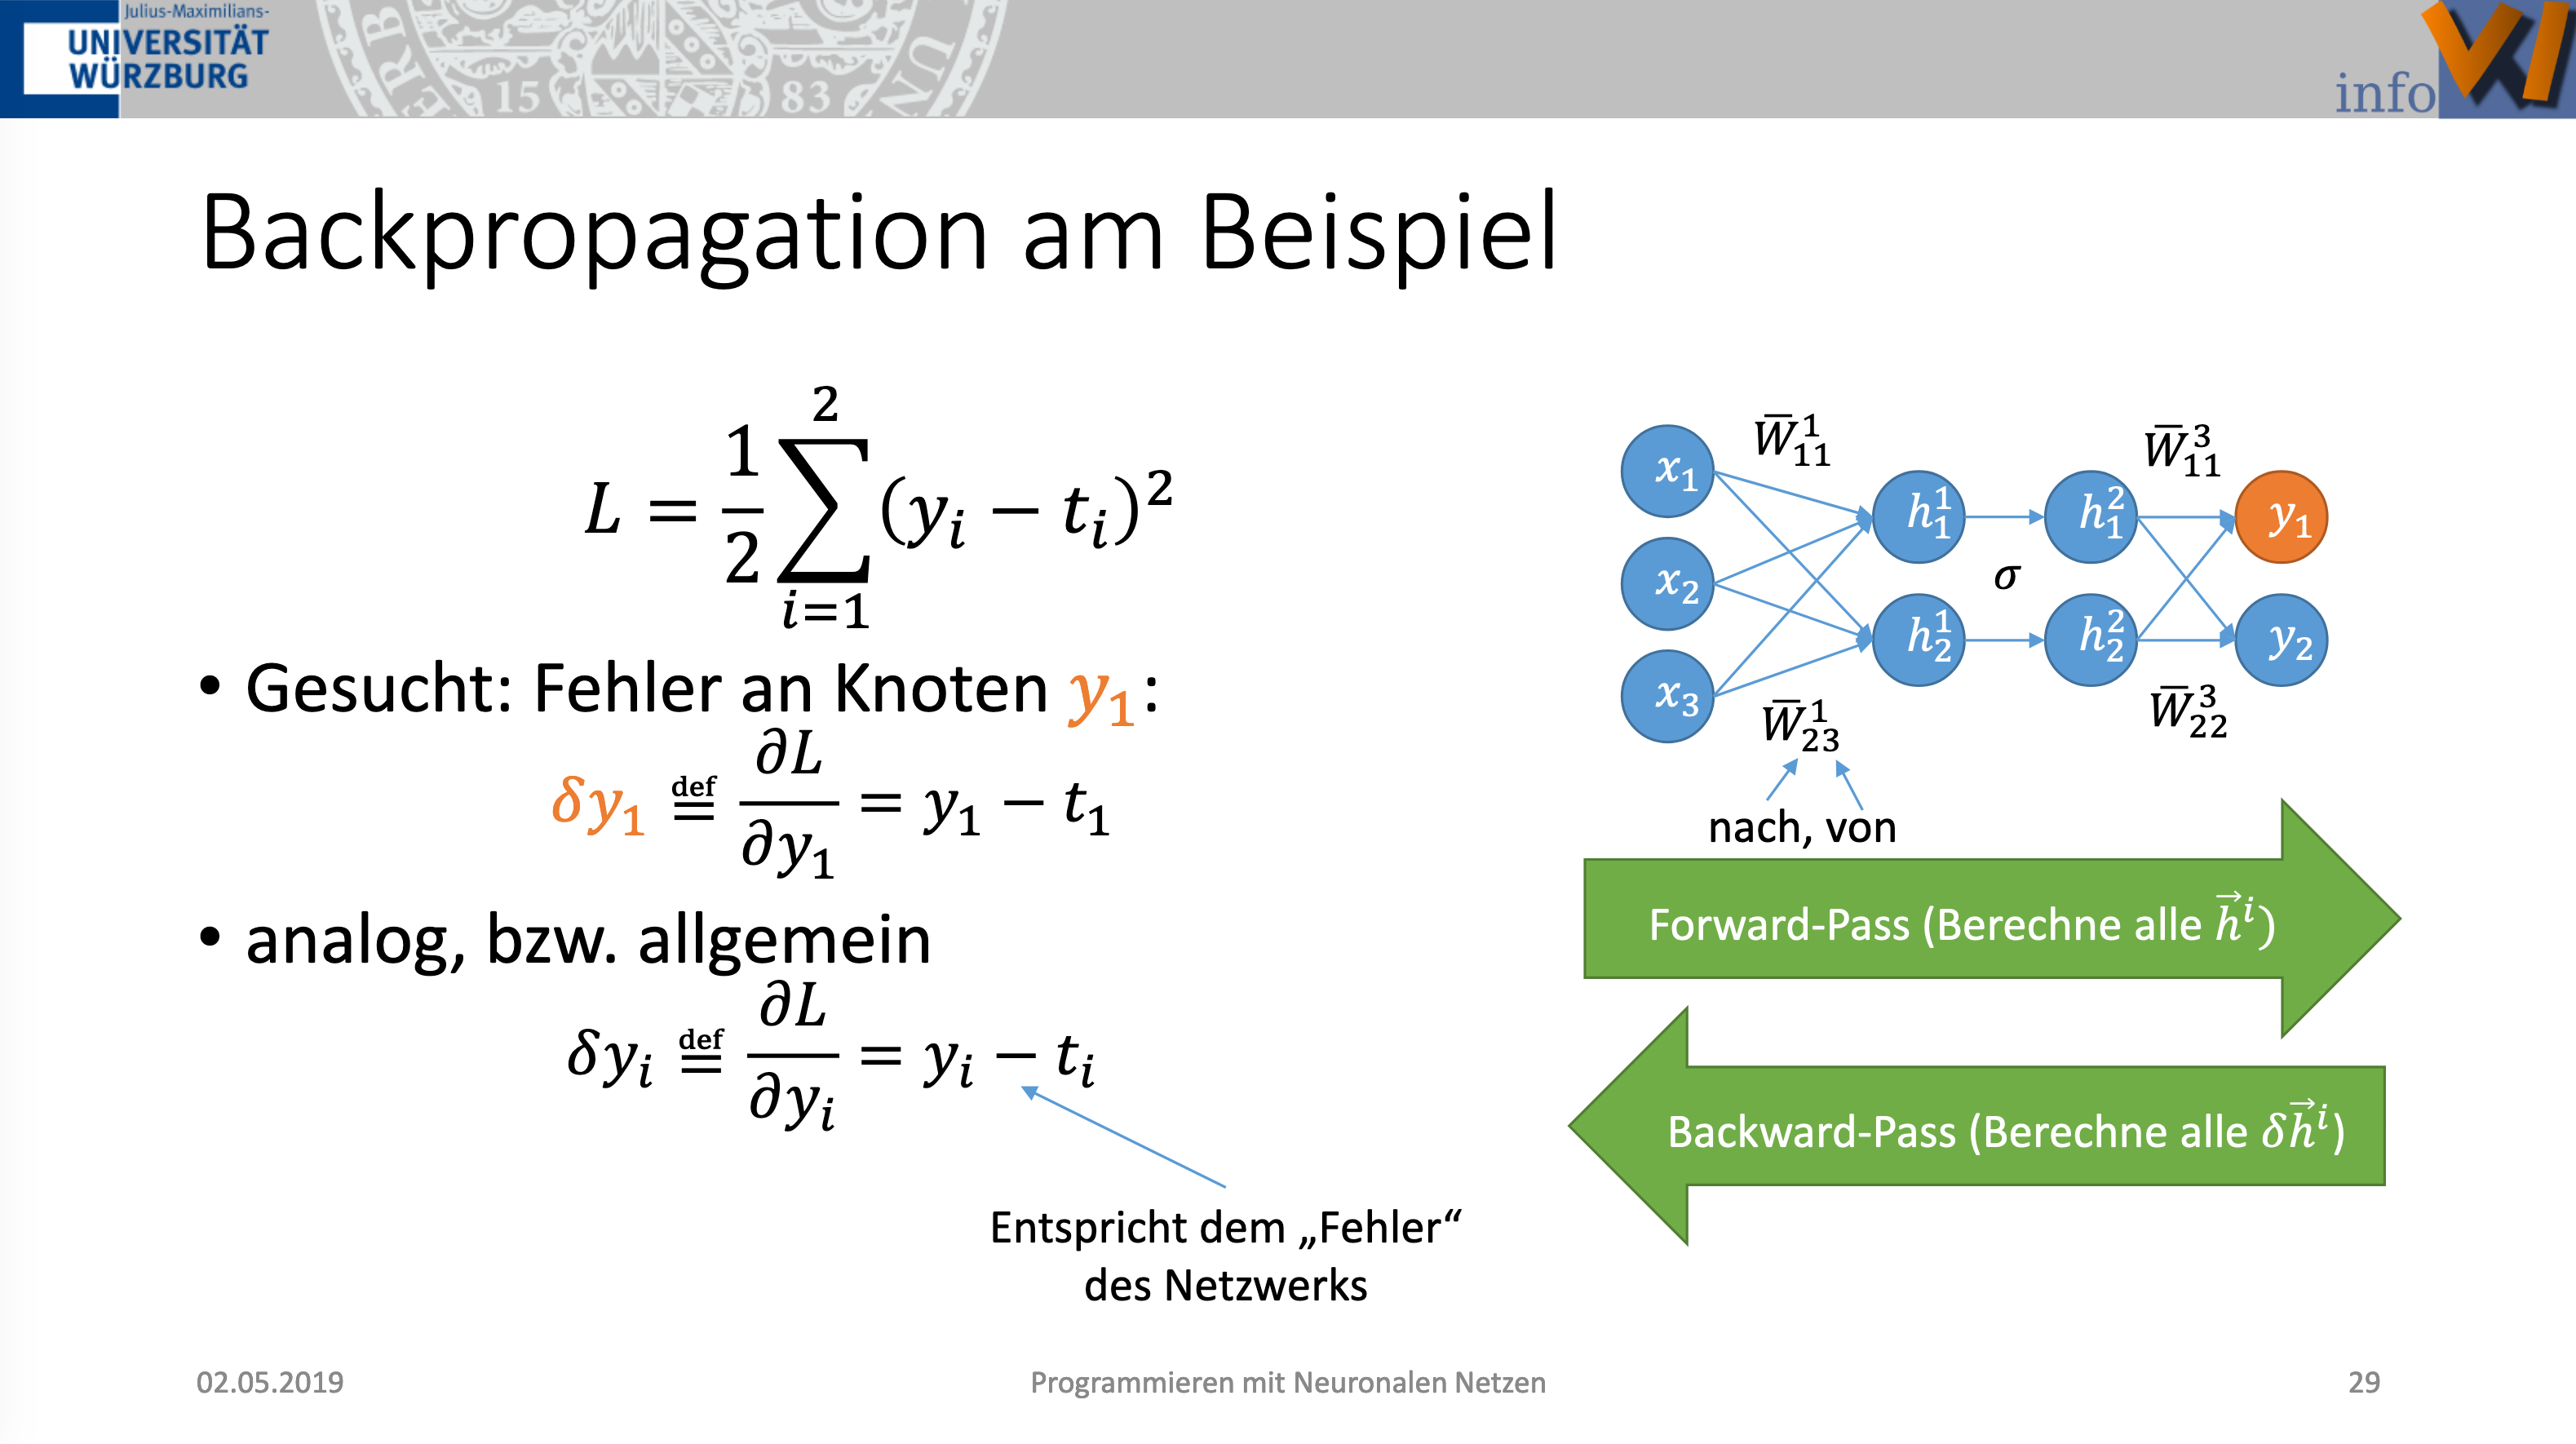
\includegraphics[width=\linewidth]{figures/backpropagation.png}\\
	\textbf{Berechnung der Gewicht-Deltas} Bilden der partiellen Ableitung für jedes Gewicht jedes Layers und Speichern der Werte als Deltas. Zur Berechnung sind die Deltas der Outputs (siehe Backward-Pass) erforderlich. Für Batches werden die Deltas der Gewichte aufsummiert und nach dem Batch geupdated.\\
	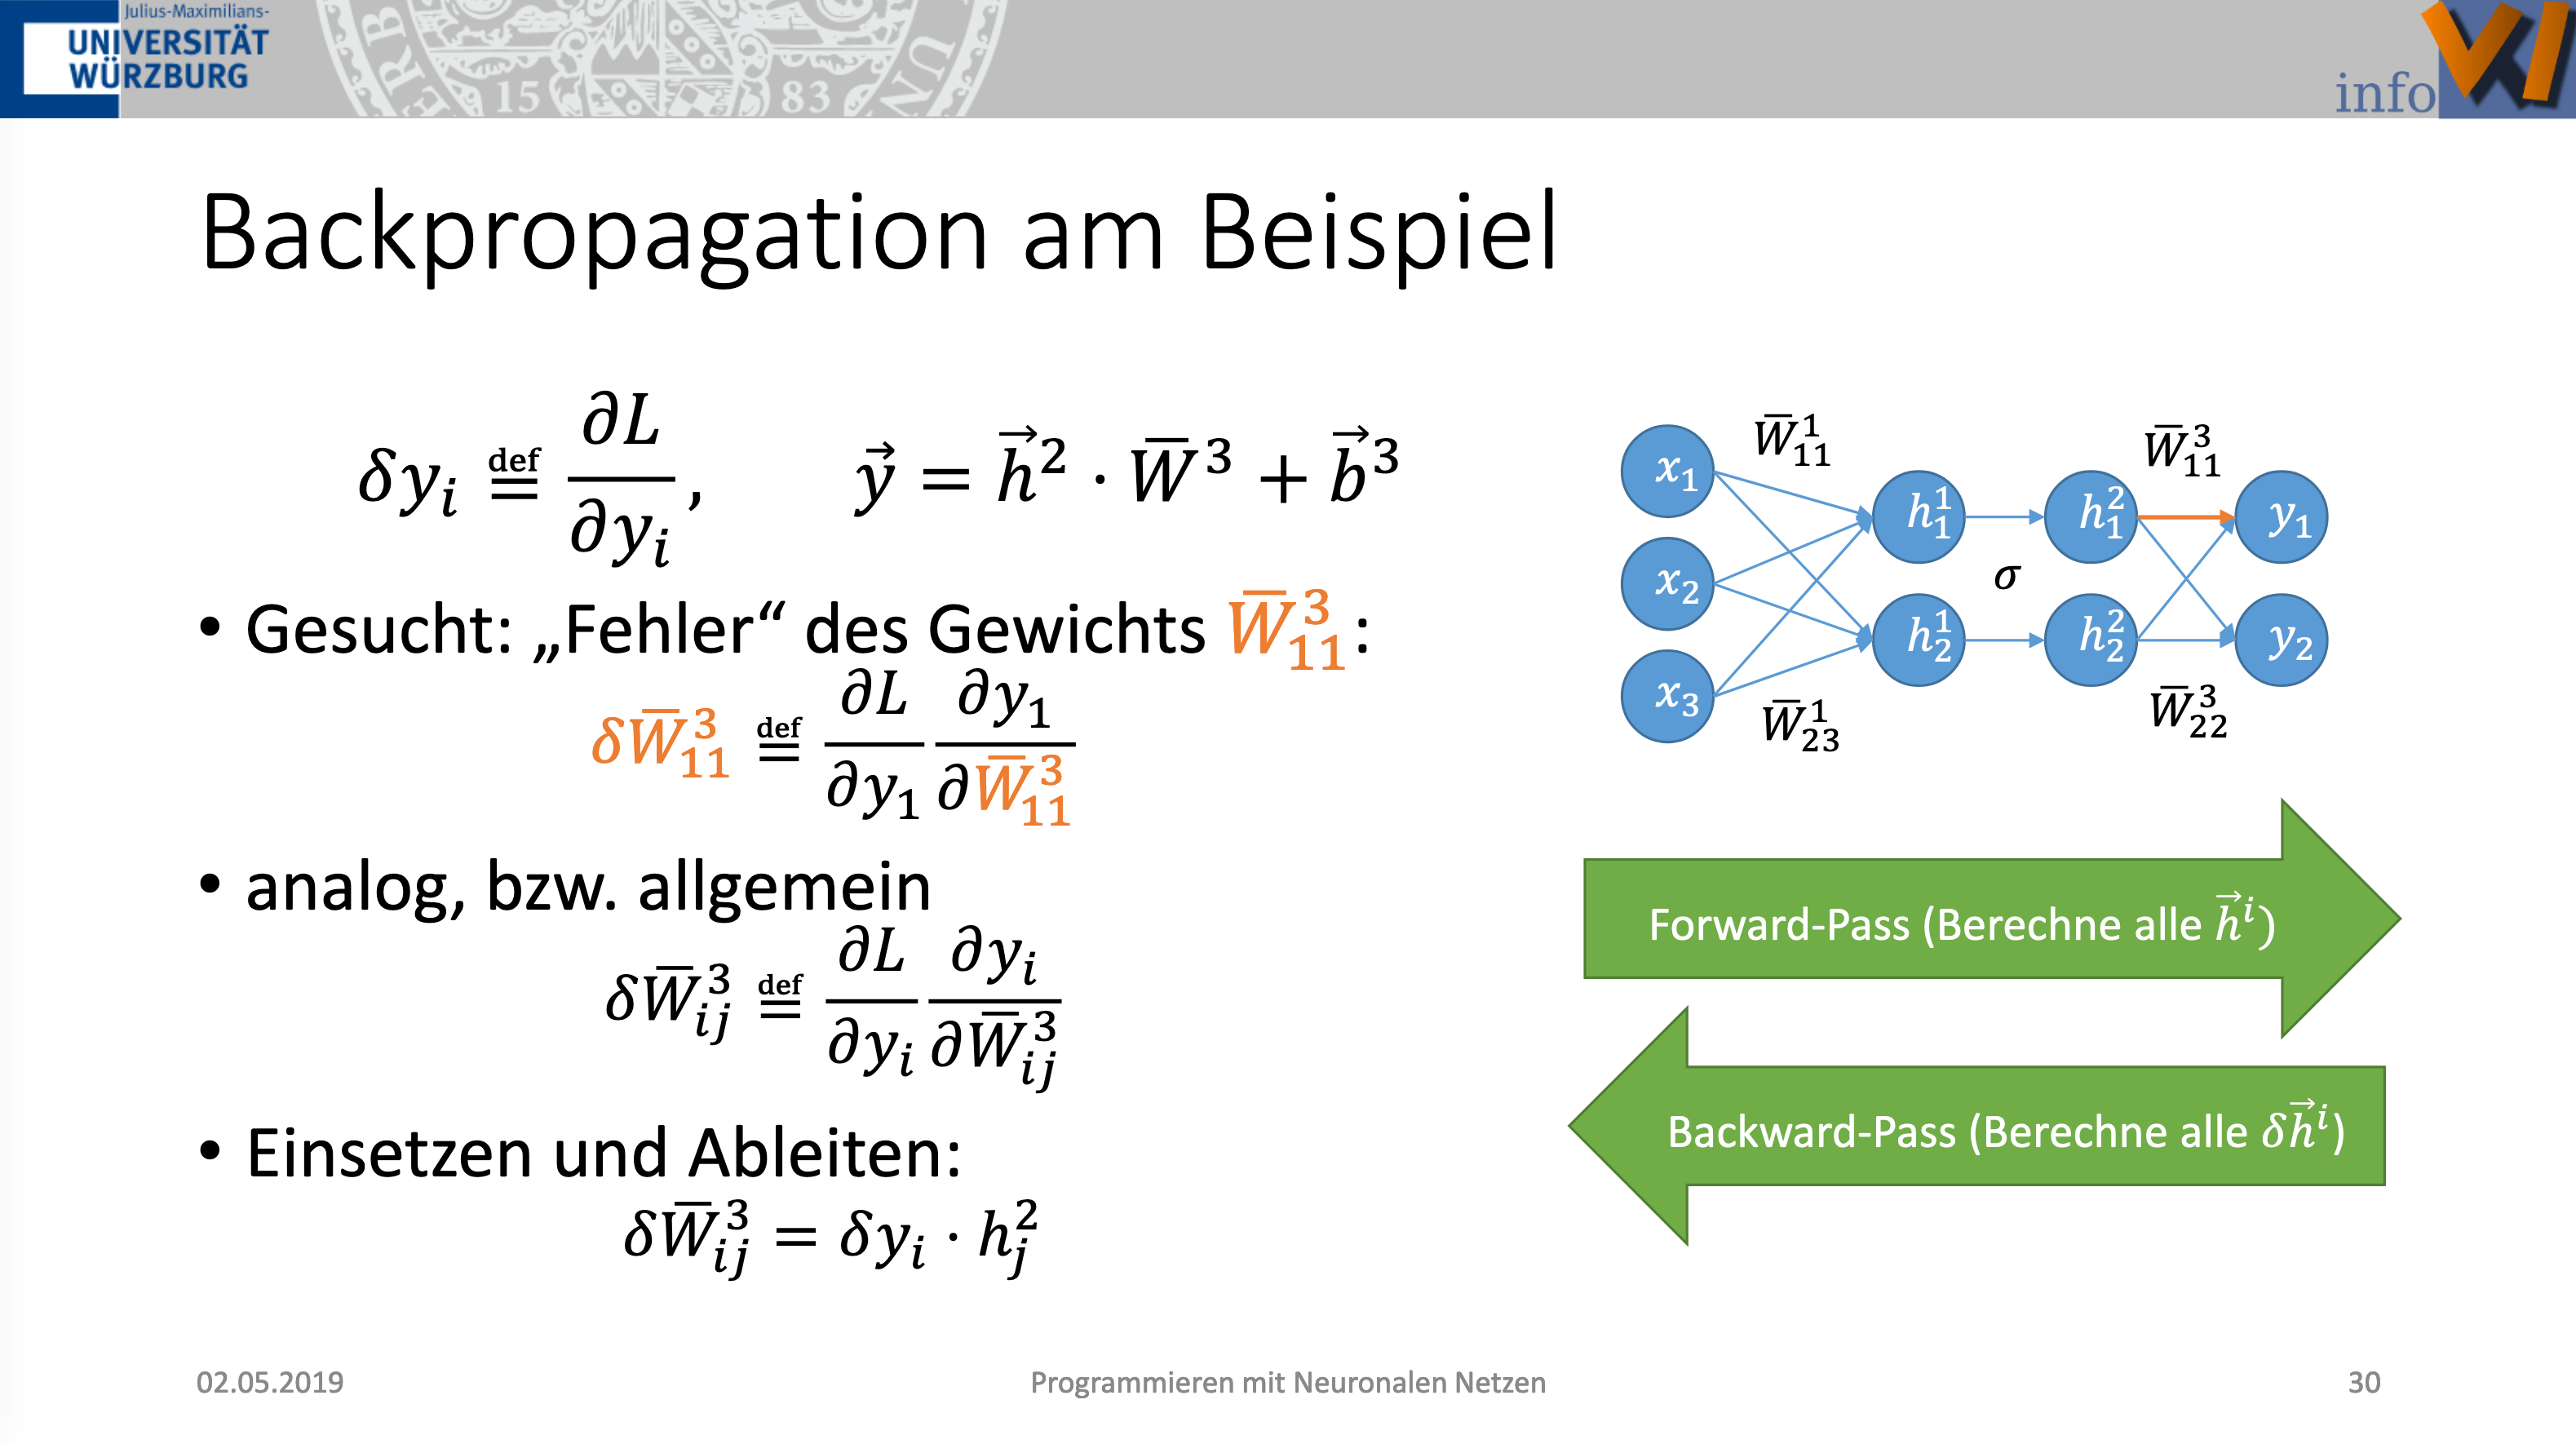
\includegraphics[width=\linewidth]{figures/calculate-delta-weights.png}\\
	\textbf{Update der Gewichte} Die Gewichte werden nun geupdated, in dem die Deltas der Gewichte mit den ursprünglichen Gewichten verrechnet werden. Dafür gibt es verschiedene Optimierungsverfahren:
	\begin{itemize}
		\item Gradient Descent: für Gewicht $w'_{ij} = w_{ij} - \eta \cdot \delta w_{ij}$
		\item Adam-Optimizer: robuster gegeüber schlecht gewählter Learning-Rate
		\item Adagrad
		\item RMSProp
	\end{itemize}
	\textbf{Regularisierung} Methoden um Overfitting vorzubeugen
	\begin{itemize}
		\item Rauschen auf Eingabedaten, Gewichten, Ausgabe (Zufallswerte hinzufügen)
		\item Datenaugmentierung
		\item Early-Stopping: Laufende Validierung auf Validierungsset, Trainingsabbruch wenn Accuracy abnimmt
		\item Dropout (siehe Layer)
		
	\end{itemize}
	\textbf{Pre-Training} Verwende Startgewichte, die bereits auf ähnlichen Daten trainiert wurden $\rightarrow$ besser als zufällige Initialisierung.\\
	\textbf{Transferlearning} Verwende vortrainiertes Netz und trainiere nur einzelne Schichten (z.B. letzte Schicht für Klassifikation) neu.

	\subsection{Netzarchitektur}
	\textbf{Perceptron} (= künstliches Neuron) stellt lineare Trennung (binäre Klassifikation) dar. Kann Funktionen AND, OR und NOT lernen, nicht aber XOR.\\
	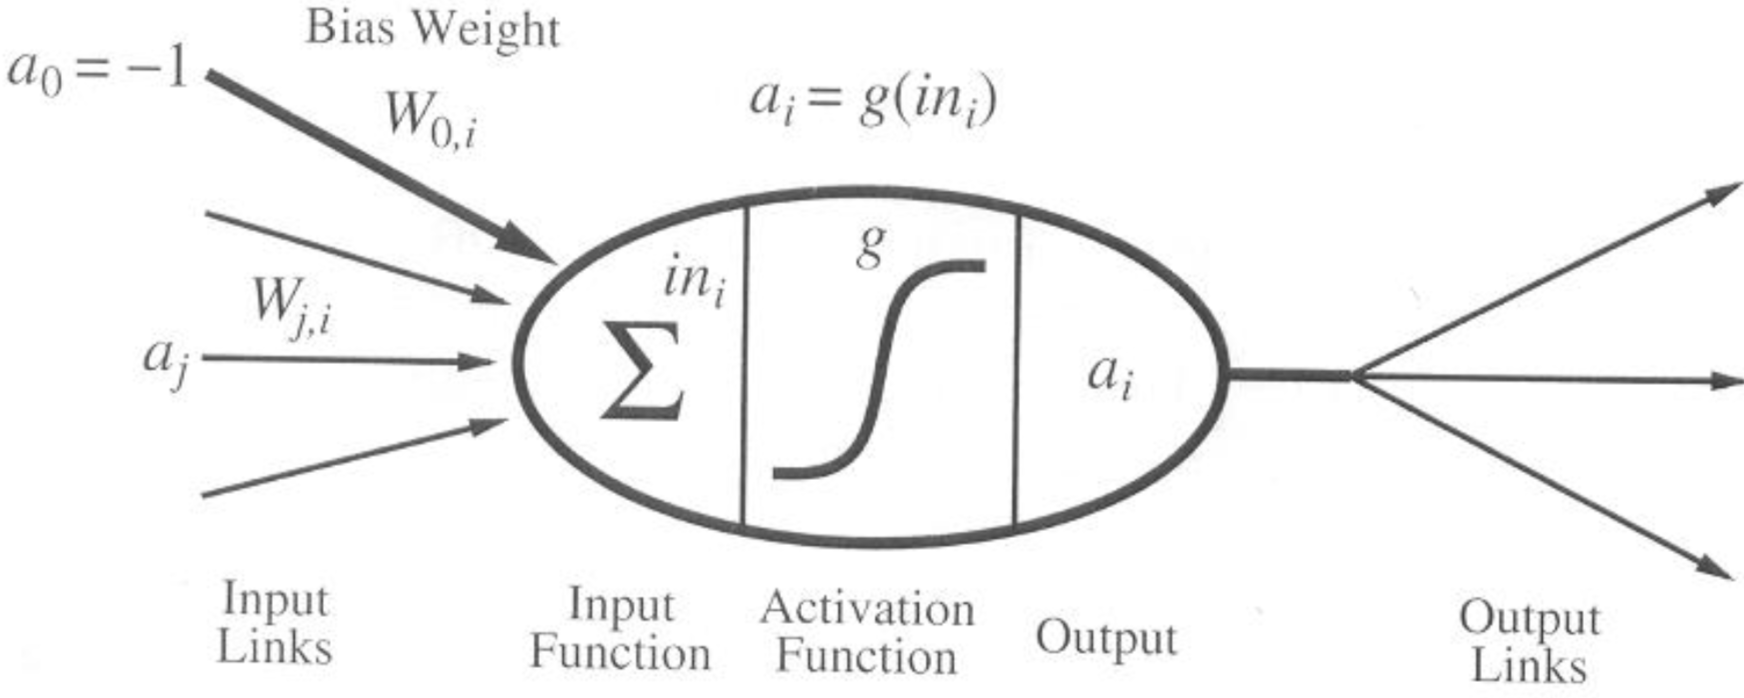
\includegraphics[width=\linewidth]{figures/perceptron.png}\\
	mit Inputs $a_j$ gewichtet mit $W_{ji}$ (ergeben zusammen die Gewichtsmatrix $W$), addiert mit Bias $b$, Outputs $a_i$ und der Aktivierungsfunktion $g$ mit der der Output berechnet wird.
	$$Ausgabe_{Schicht(x)} = g(Eingabe_{Schicht(x)} \cdot W + b) = Eingabe_{Schicht(x+1)}$$
	\textbf{Aktivierungsfunktion} muss bei Multi-Layer-Perceptronen (MLP) nicht-linear sein, da sonst nicht mehr Information gespeichert werden kann.
	$$(x \cdot W + b) \cdot V + a = x \cdot W \cdot V + b \cdot V + a = x \cdot W' + b'$$

	\section{Layer}
	Mögliche Schichten aus denen ein neuronales Netz bestehen kann.
	\subsection{Fully Connected / Dense}
	Voll verbundene Schicht, d.h. jeder Input landet in jedem Neuron. Wird z.B. als letzter Layer zur Klassifikation verwendet, um Vektor mit Logits für Klassen auszugeben.\\
	\textbf{Parameter} $X \in \R^{1 \times a}$: Eingabe, $W \in \R^{a \times n}$: Gewichtsmatrix, $b \in \R^{1 \times n}$: Bias, $n$: Anzahl der Neuronen, $Y \in \R^{1 \times n}$: Ausgabe\\
	\textbf{Forward-Pass} $$Y = X \cdot W + b$$
	\textbf{Backward-Pass} $$\delta X = \delta Y \cdot W^T$$
	\textbf{Calculate Delta Weights} $$\frac{\delta L}{\delta W} = X^T \cdot \delta Y$$ $$\frac{\delta L}{\delta b} = \delta Y$$
	\subsection{Aktivierungsfunktion}
	Elementweise Anwendung\\
	\begin{tabular}{|l|l|l|}
	\hline
	\textbf{Funktion} & \textbf{Forward} & \textbf{Backward}\\
	\hline
	tanh & $Y = \tanh(X)$ & $\delta X = (1 - \tanh^2(X)) \odot \delta Y$\\
	\hline
	Sigmoid & $Y = \sigma(X) = \frac{1}{1 + e^{-X}}$ & $\delta X = (\sigma(X) \cdot (1-\sigma(x))) \odot \delta Y$\\
	\hline
	ReLU & $Y = ReLU(X)$ & $\delta X = ReLU'(X) \odot Y$\\
	\hline
	\end{tabular}\\
	\\
	ReLU: $ReLU(x) = x > 0 ? x : 0$, $ReLU'(x) = x > 0 ? 1 : 0$
	\subsection{Softmax}
	Normalisiert eine Menge von Werten, sodass deren Summe 1 ergibt. Wird zur Berechnung der Wahrscheinlichkeitsverteilung bei Klassifikation verwendet.\\
	\textbf{Forward-Pass} $$Y = softmax(X) = \frac{e^{x_i}}{\sum_i e^{x_i}}$$
	\textbf{Backward-Pass} $$\delta X = \delta Y \cdot
	\begin{bmatrix}
	\frac{\delta y_1}{\delta x_1} & \cdots & \frac{\delta y_n}{\delta x_1}\\
	\cdots & \ddots & \cdots\\
	\frac{\delta y_1}{\delta x_n} & \cdots & \frac{\delta y_n}{\delta x_n}
	\end{bmatrix}
	$$
	\subsection{Dropout}
	Für Regularisierung verwendet. Ein Teil der Gewichte wird zufällig je Durchlauf auf 0 gesetzt (deaktiviert). Wird nicht trainiert, sollten alle Gewichte weitergegeben, aber durch die Dropout-Rate geteilt werden, da sonst eine zu hohe Aktivierung der nächsten Schicht statt findet.\\
	\textbf{Parameter} $d$: Dropout-Rate gibt den prozentualen Anteil der zu deaktivierenden Gewichte an.
	\subsection{Convolutional}
	Extrahiert Features aus einer Matrix. Wird oft in der Bildklassifizierung verwendet oder NLP zur Satzklassifikation (Kernel Größe der Embeddings $\times$ Anzahl betrachteter Wörter).\\
	\textbf{Parameter}\\
	$X \in \R^{h \times w \times d}$: Eingabe\\
	$(fh, fw)$: Filtergröße\\
	$fn$: Anzahl Filter\\
	$F \in \R^{fh \times fw \times fd \times fn}$: Filtertensor\\
	$b \in \R^{fn}$: Bias (ein Wert pro Ausgabechannel, wird auf jeden Wert des Channels addiert)\\
	$Y \in \R^{(h-fh+1) \times (w-fw+1) \times fn}$: Ausgabe\\
	\textbf{Optionale Parameter} Stride: wie weit der Filter verschoben wird (default = 1), Dilation: zusätzliche 0en im Filter (Filter über nicht benachbarte Elemente)\\
	\textbf{Padding} Covolution verkleinert die Daten. Um dies zu verhindern, kann die Eingabe gepadded werden (Hinzufügen von 0en am Rand der Eingabe).\\
	\textit{Half-Padding}: Ausgabegröße = Eingabegröße, $ph = \lfloor \frac{fh}{2} \rfloor$, $pw = \lfloor \frac{fw}{2} \rfloor$\\
	\textit{Full-Padding (Full-Convolution)}: Ausgabegröße $>$ Eingabegröße, $ph = fh - 1$, $pw = fw - 1$\\
	\textbf{Forward-Pass} $*$ bezeichnet die Faltungsoperation\\
	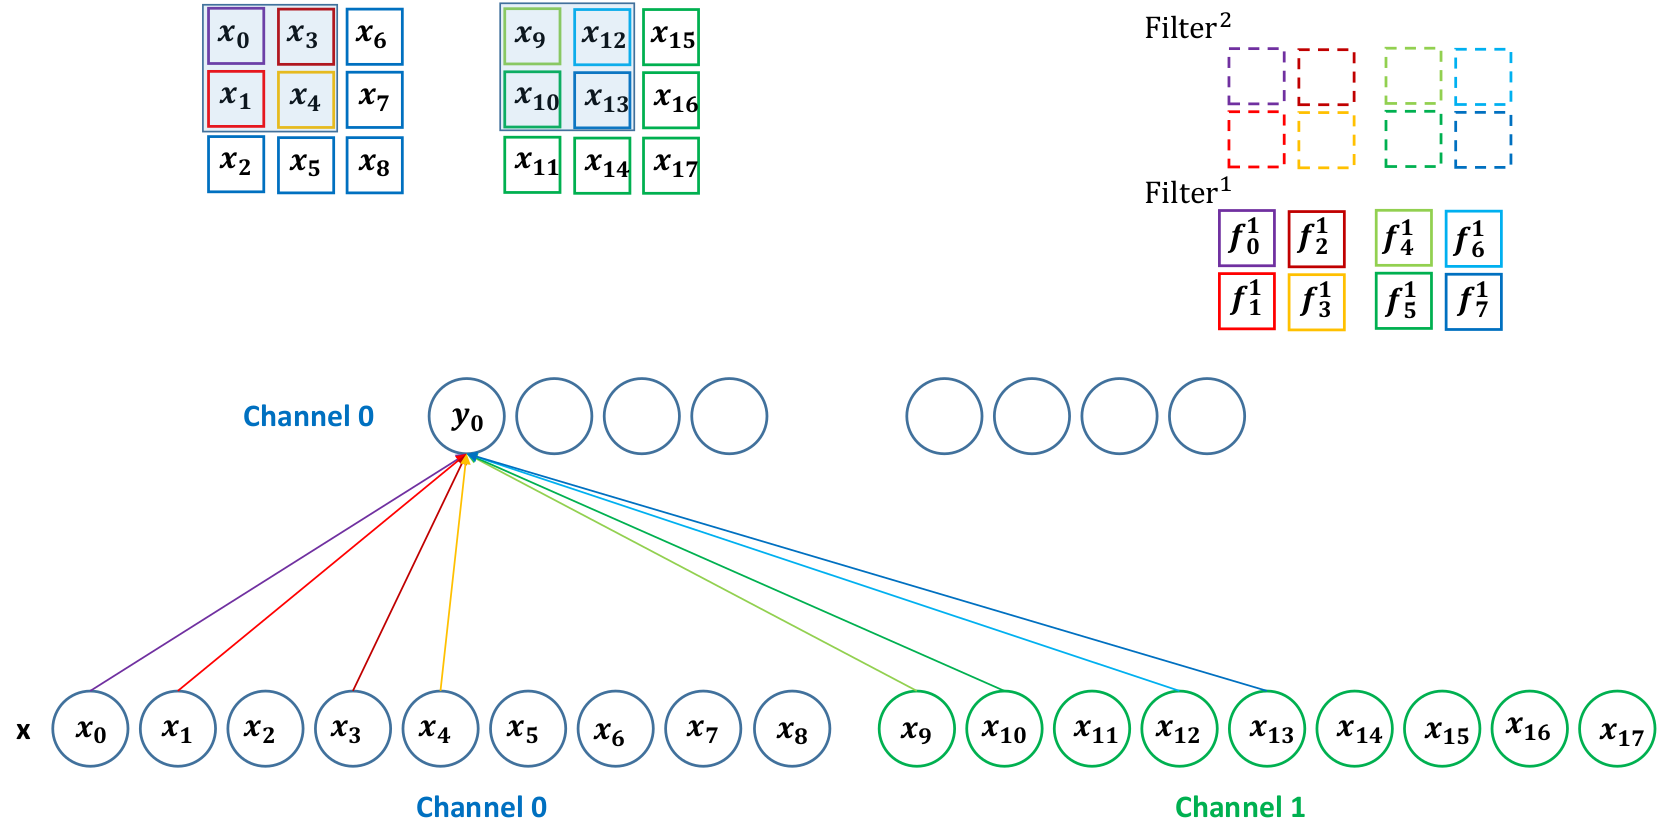
\includegraphics[width=\linewidth]{figures/convolution.png}
	$$Y = X * F + b$$
	\textbf{Backward-Pass} $*_F$ bezeichnet die Full-Convolution\\
	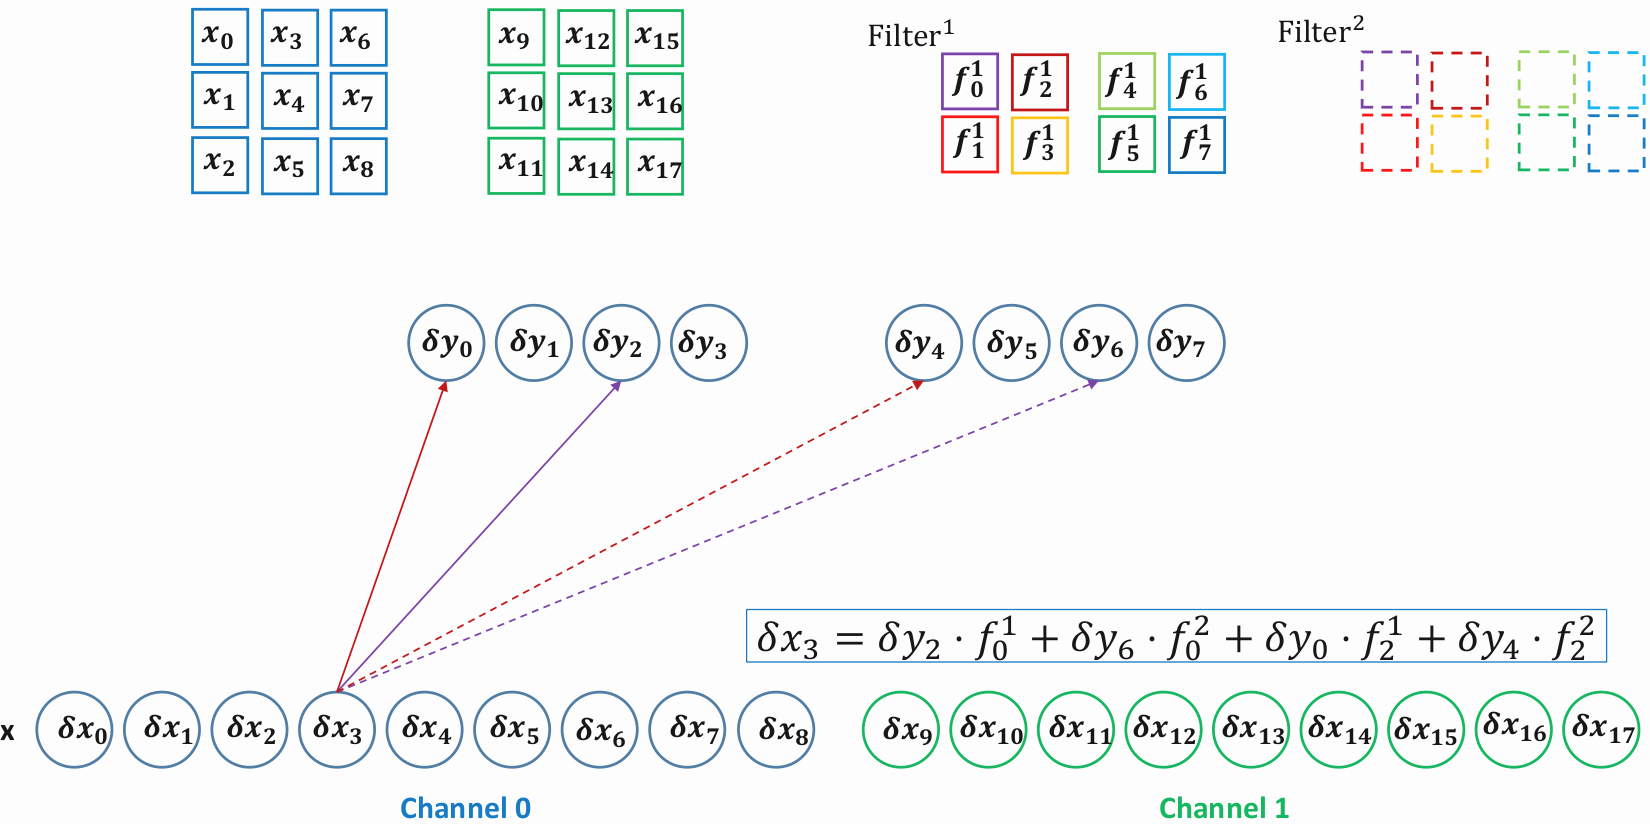
\includegraphics[width=\linewidth]{figures/convolution-backward.png}
	$$\delta X = \delta Y *_F rot^{180}_{h,w}(trans(F))$$
	\textbf{Calculate Delta Weights} $*_{ch}$ bezeichnet die Channel-Wise-Convolution, $f$ ist ein Element des Filtertensors
	$$\frac{\delta L}{\delta f} = X *_{ch} \delta Y$$
	$$\frac{\delta L}{\delta b_f} = \sum_i \delta y_{i,f}$$
	\subsection{Pooling}
	Reduziert die Werte innerhalb eines Filters auf einen Wert (z.B. Maximum oder Durchschnitt). Filter wird ohne Überlappung (mit Stride) verschoben.\\
	\textbf{Forward-Pass}\\
	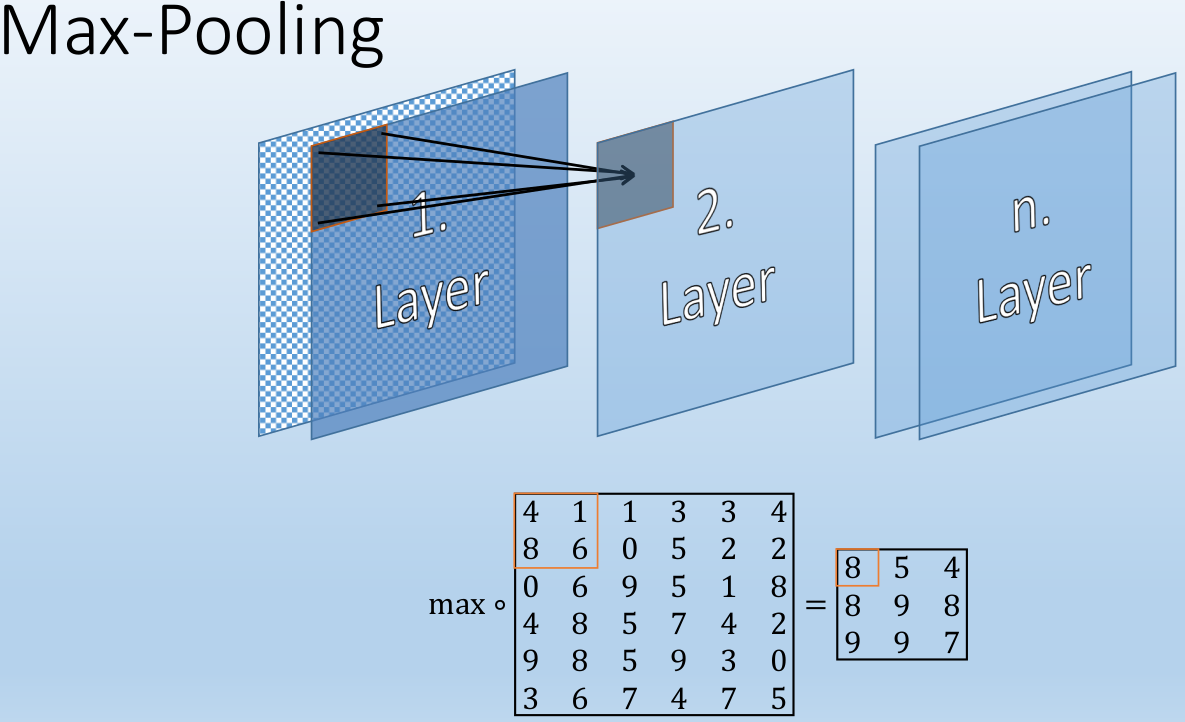
\includegraphics[width=\linewidth]{figures/max-pooling.png}\\
	\textbf{Backward-Pass} Nur die Elemente, die im Forward-Pass an der Berechnung des Outputs beteiligt waren, bekommen anteilig oder ganz das Delta des jeweiligen Outputs.
	$$\delta x_i = (x_i == max) ? \delta y : 0$$
	\subsection{Vanilla RNN}
	Recurrent Neuronal Networks (RNNs) werden verwendet, um Daten unterschiedlicher Länge zu verarbeiten. Dabei wird ein Hidden State $h$ in jedem Schritt um Informationen der Eingabe ergänzt.\\
	\textbf{Parameter}\\
	$[x_0, \cdots, x_n] = X \in \R^{n \times m}$: Eingabevektoren mit jeweils Länge $m$\\
	$g$: Zwischenvariable nach der Addition vor $\tanh$\\
	$h$: Hidden State ($h_{-1}$ kann mit Nullen initialisiert werden)\\
	$W_x, W_h, W_o$: Gewichtsmatrizen\\
	$b$: Bias\\
	$[o_0, \cdots, o_n] = O \in \R^{n \times l}$: Ausgabevektoren mit jeweils Länge $l$\\
	\textbf{Funktionsweise}\\
	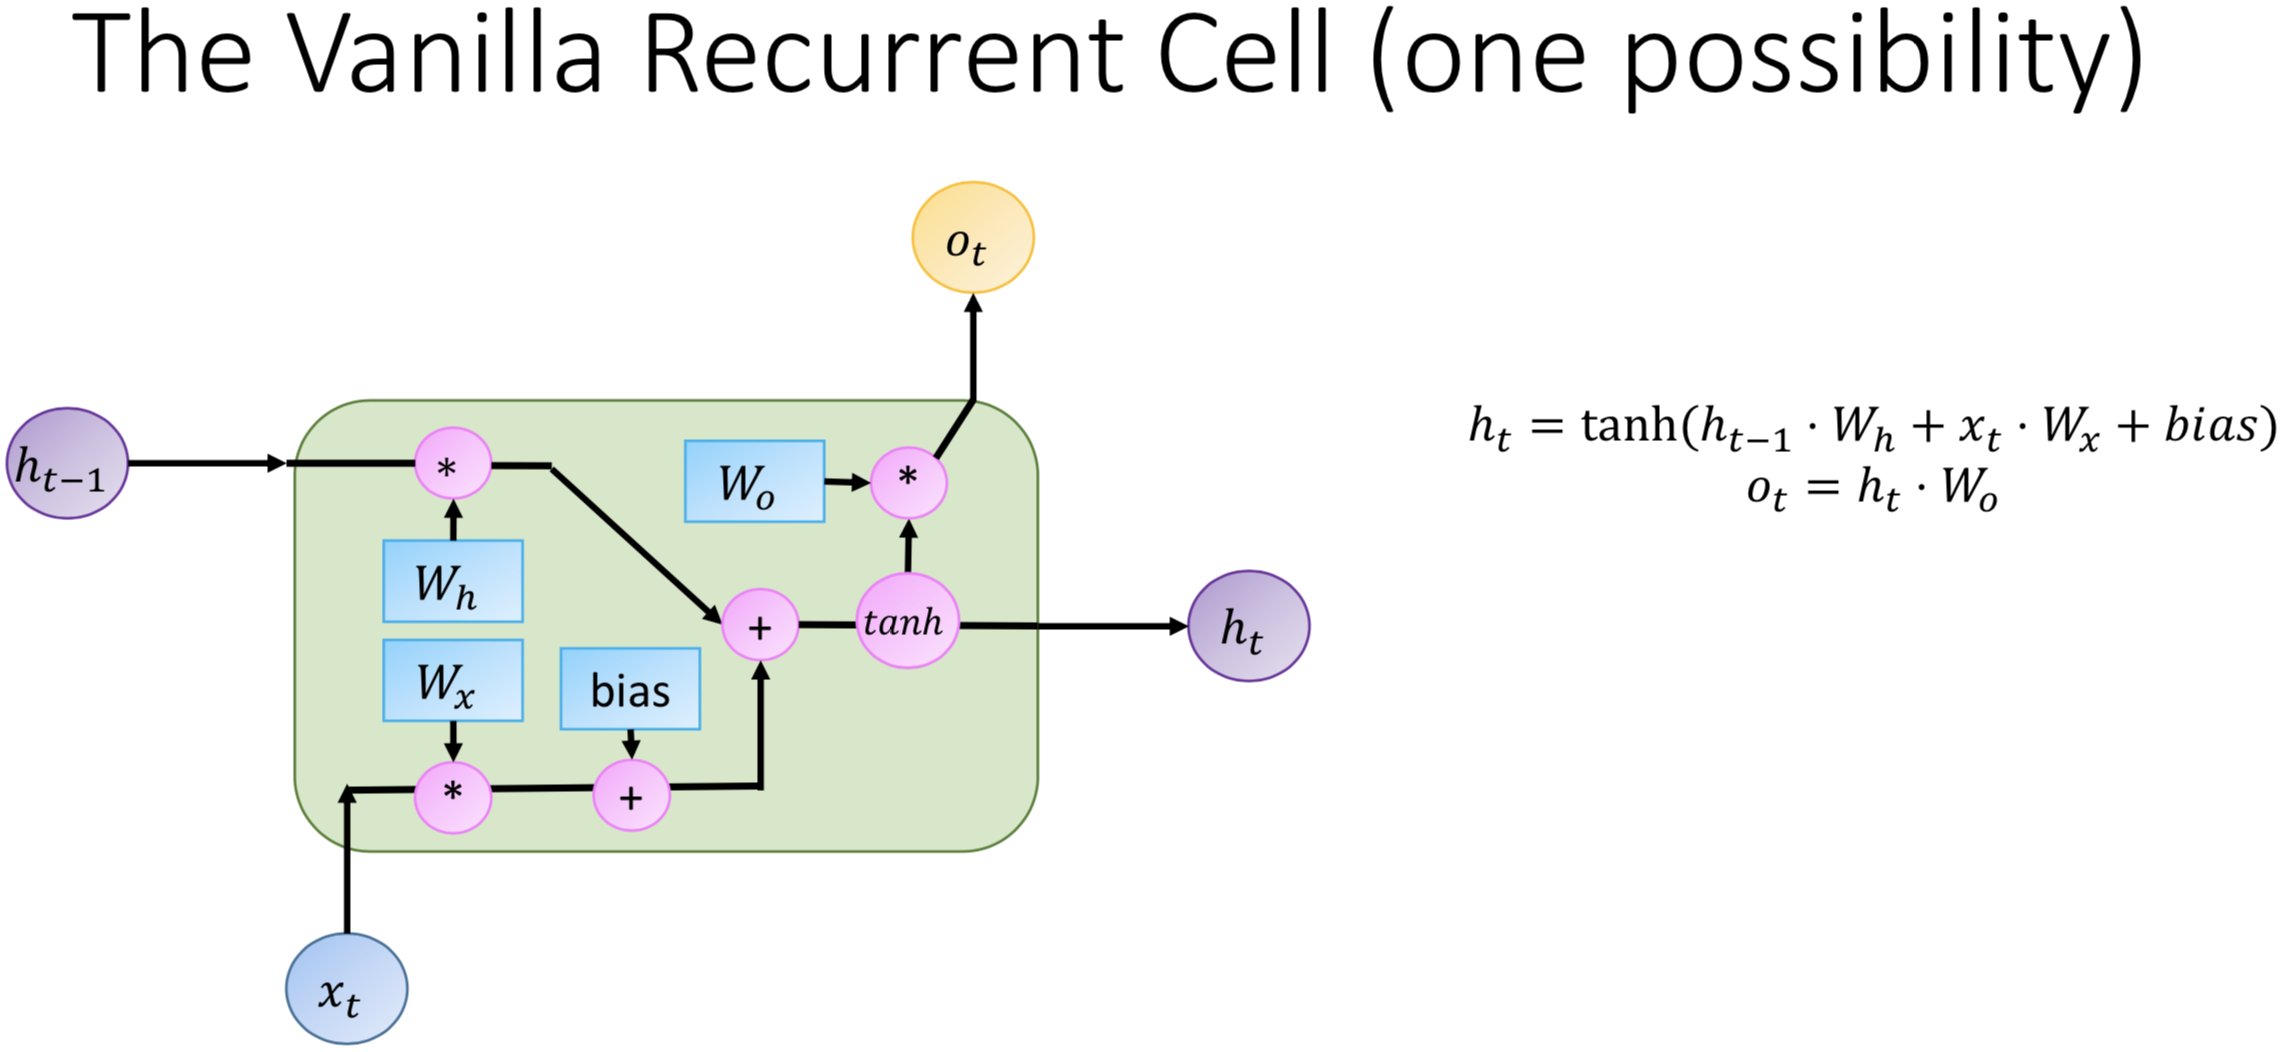
\includegraphics[width=\linewidth]{figures/vanilla-rnn.png}\\
	\textbf{Forward-Pass}
	$$h_t = \tanh(h_{t-1} \cdot W_h + x_t \cdot W_x + b)$$
	$$o_t = h_t \cdot W_o$$
	\textbf{Backward-Pass}
	$$\delta h_t = \delta o_t \cdot W_o^T + \delta g_{t+1} \cdot W_h^T$$
	$$\delta g_t = \delta h_t \cdot (1 - \tanh^2(g_t)) = \delta h_t \cdot (1 - h_t^2)$$
	$$\delta x_t = \delta g_t \cdot W_x^T$$
	\textbf{Calculate Delta Weights}
	$$\delta W_h = \sum_t h_{t-1}^T \cdot \delta g_t$$
	$$\delta W_x = \sum_t x_t^T \cdot \delta g_t$$
	$$\delta W_o = \sum_t h_t^T \cdot \delta o_t$$
	$$\delta b = \sum_t \delta g_t$$
	\subsection{Gru}
	Verwendet zwei Gates (wie $g$ im Vanilla RNN), um zu bestimmen, was aus dem alten Internal State $h$ übernommen wird und was von den aktuell verarbeiteten Daten hinzugefügt wird.\\
	\textbf{Funktionsweise}\\
	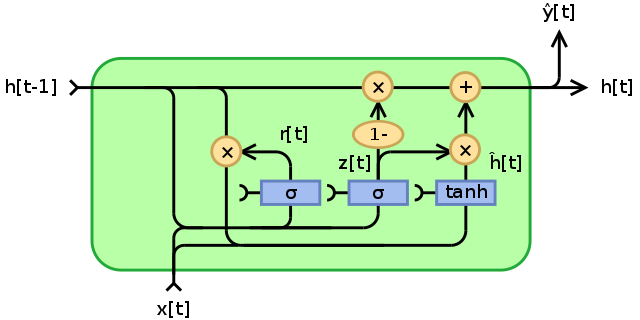
\includegraphics[width=\linewidth]{figures/gru.png}
	\subsection{LSTM}
	Verwendet drei Gates (Forget, Input, Output) und zusätzlichen State $c$\\
	\textbf{Funktionsweise}\\
	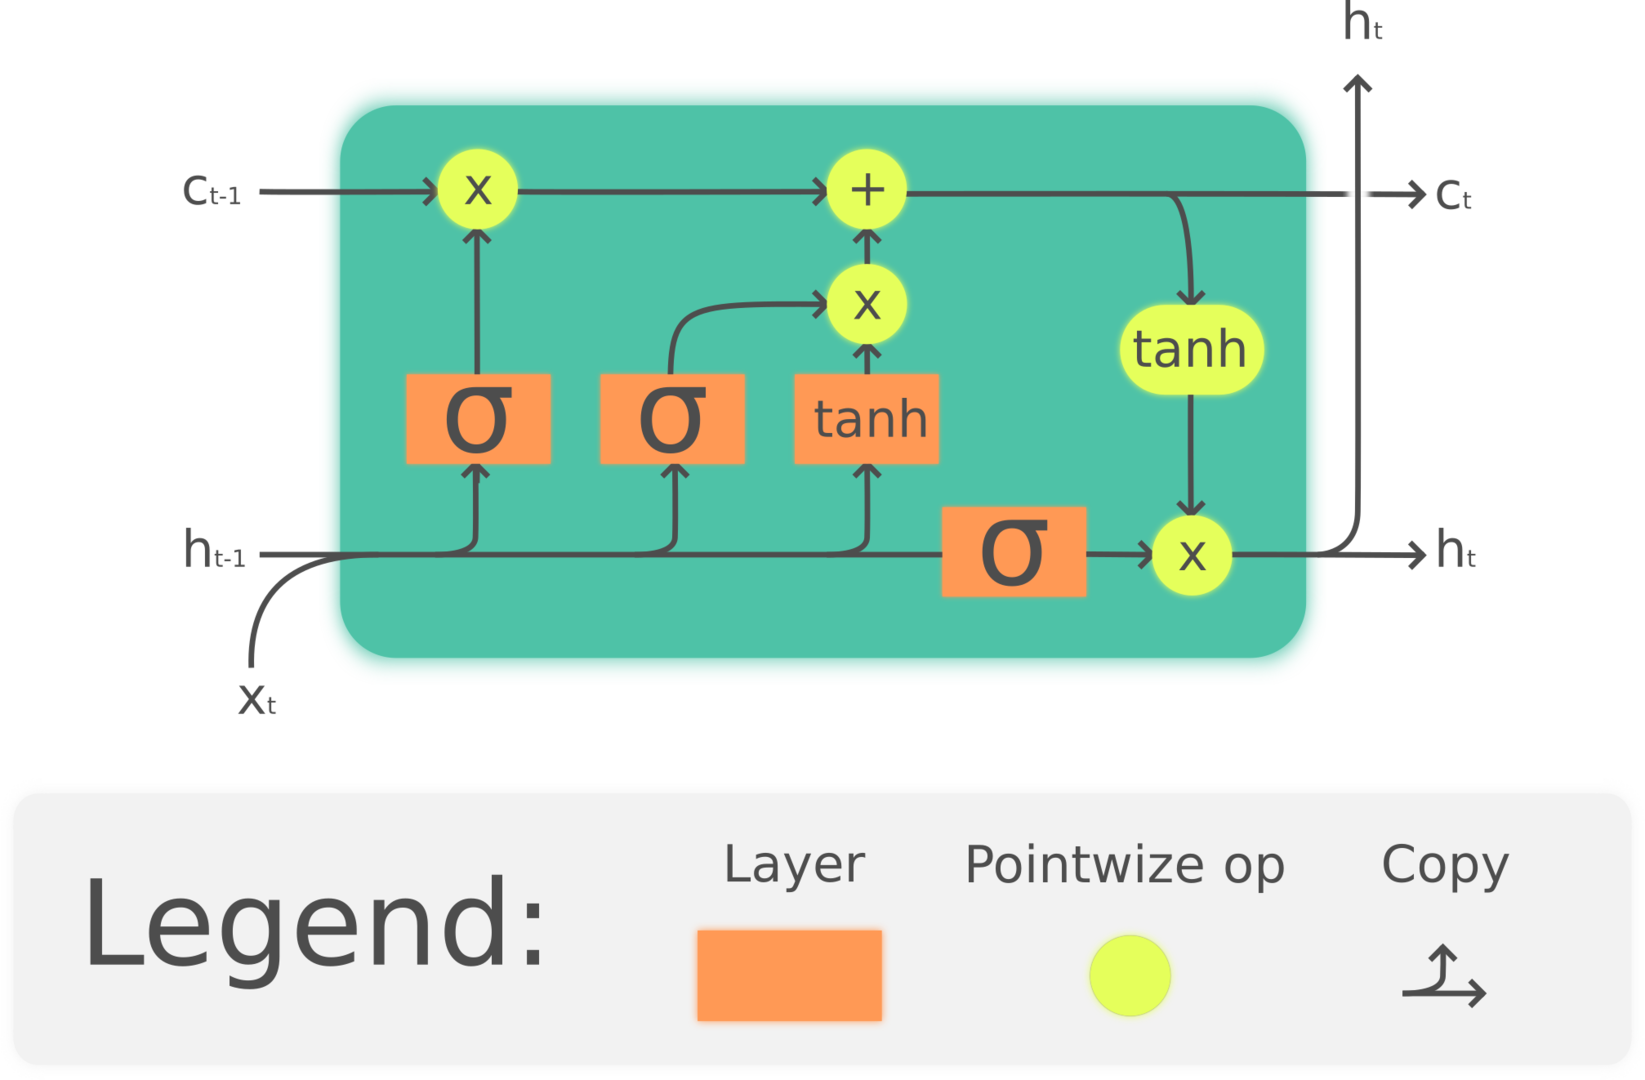
\includegraphics[width=\linewidth]{figures/lstm.png}
	\subsection{Highway Layer}
	Verwendet ein Gate, das bestimmt, ob der Layer wie ein Fully Connected Layer funktioniert oder lediglich den Input weitergibt. Wird verwendet bei sehr tiefen Netzwerken ($>$ 100 Layer), um Daten über lange Zeit/viele Layer hinweg nutzbar zu machen.\\
	\textbf{Forward-Pass}
	$$Y = (X \cdot W + b) \cdot T(x) + x \cdot (1 - T(x))$$
	$$T(x) = \sigma(x \cdot W_T + b_T)$$

	\section{Loss-Funktionen}
	$X$: Eingabe der Loss-Funktion bzw. Ausgabe des Netzes (Prediction)\\
	$T$: Erwartetes Ergebnis (Ground Truth)
	\subsection{Cross Entropy}
	Negative-Log-Likelihood, Cross-Entropy\\
	\textbf{Forward-Pass} $$L = -\sum_i t_i \cdot \log(x_i)$$
	\textbf{Backward-Pass} $$\frac{\delta L}{\delta x_i} = -\frac{t_i}{x_i}$$
	\subsection{Mean Squared Error}
	Euklidischer Loss, Mean-Squared-Error, $l_2$-Loss\\
	\textbf{Forward-Pass} $$L = \sum_i \frac{1}{2} (x_i - t_i)^2$$
	\textbf{Backward-Pass} $$\frac{\delta L}{\delta x_i} = x_i - t_i$$

	\section{Bildverarbeitung}
	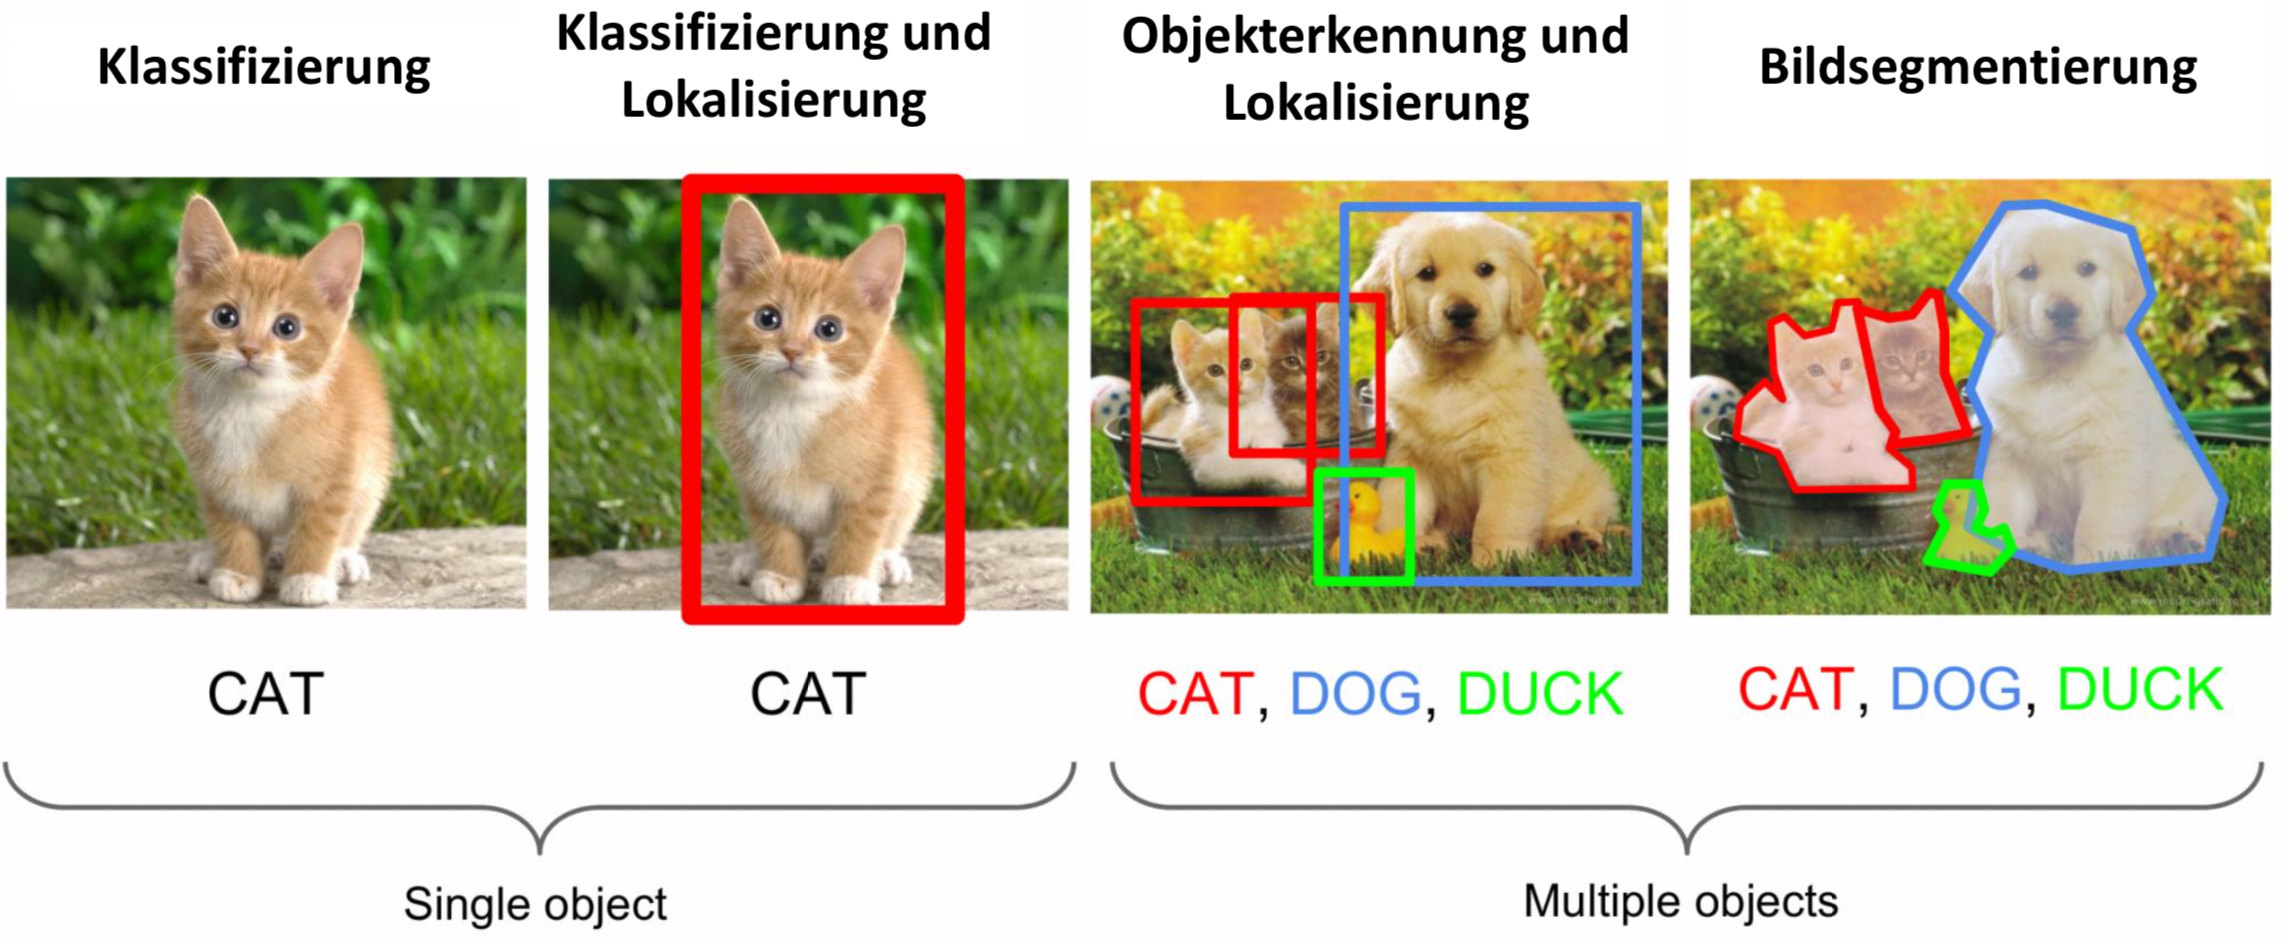
\includegraphics[width=\linewidth]{figures/bildverarbeitung.png}
	\subsection{Klassifizierung}
	In der Regel neuronales Netz mit Convolution und Fully Connected Layern, das das gesamte Bild als Eingabe bekommt.
	\subsection{Segmentierung}
	Zuweisung einer Klasse für jeden Pixel eines Bildes.\\
	\textbf{Sliding Window} Klassifizere kleinere Bildausschnitte. Probleme: Keine Flächen (benachbarte Vorhersagen haben keinen direkten Einfluss), Auflösung wird niedriger durch CNN, kleiner Stride führt zu Mehrfachberechnung\\
	\textbf{Fully Convolution Network} CNN als Encoder, das Größe verkleinert. Anschließend hochskalieren (Decoder) $\rightarrow$ schnell aber ungenau\\
	\textbf{Skip Connections} Addieren/Konkatinieren mit Werten aus vorherigen Layern\\
	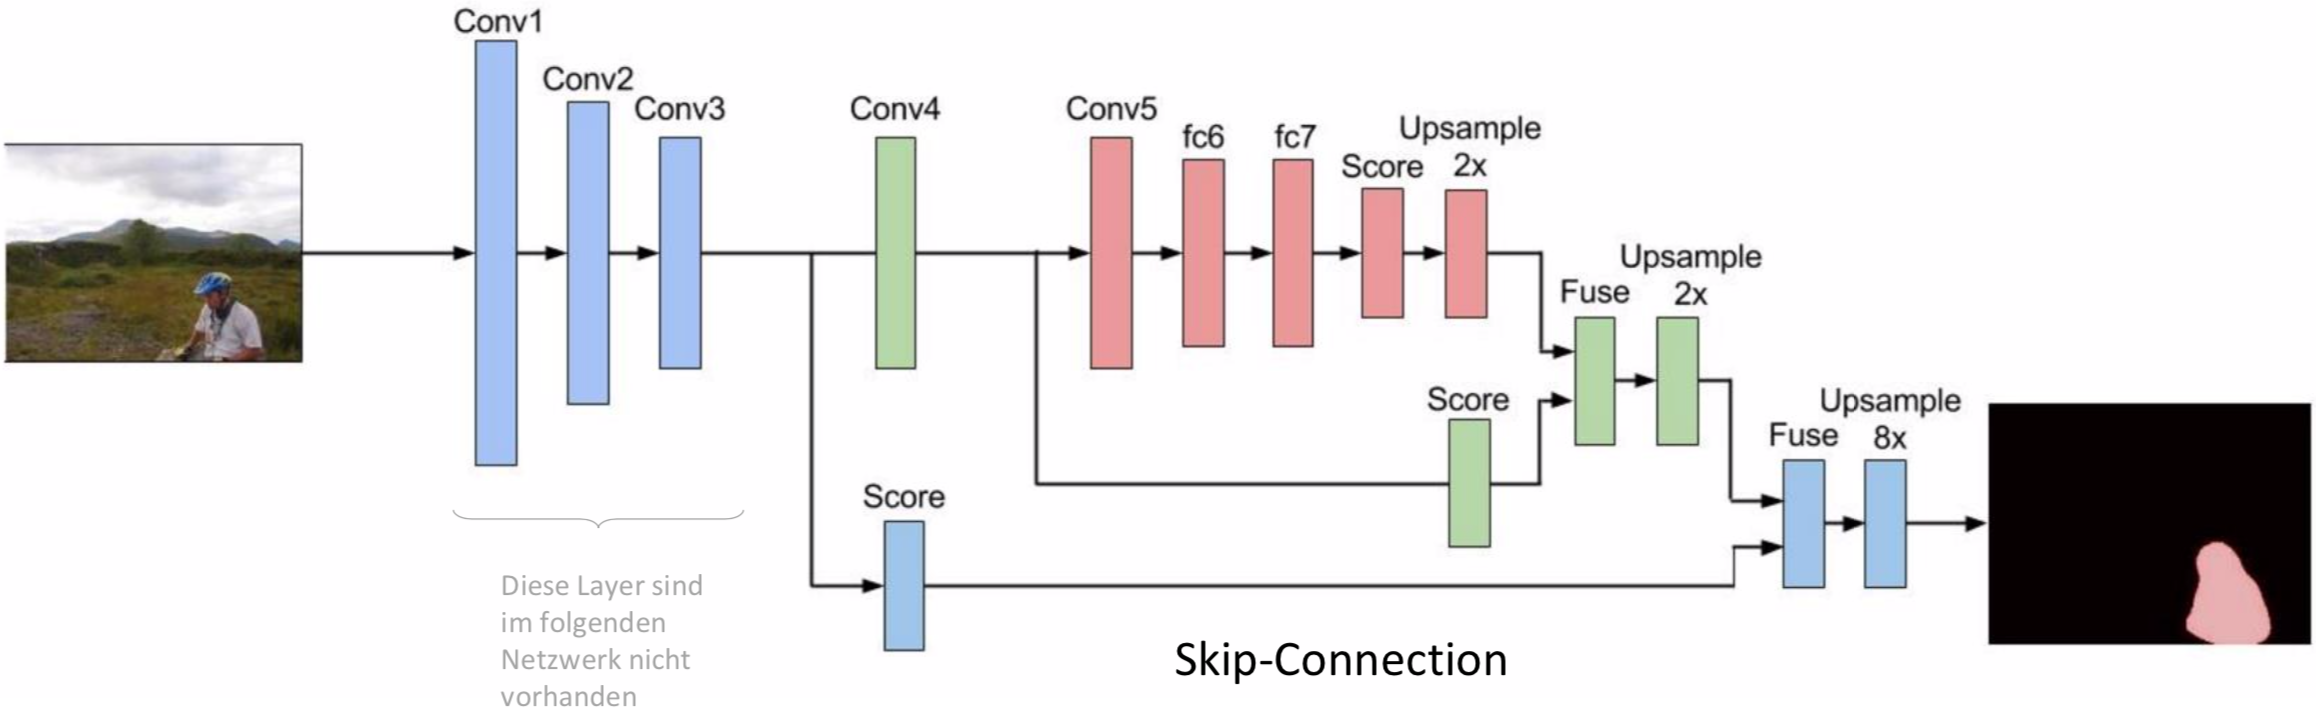
\includegraphics[width=\linewidth]{figures/skip-connections.png}\\
	\textbf{Transposed Convolution} Anwenden der transponierten Convolution zur Bildvergrößerung (wie im Backward-Pass der regulären Convolution)\\
	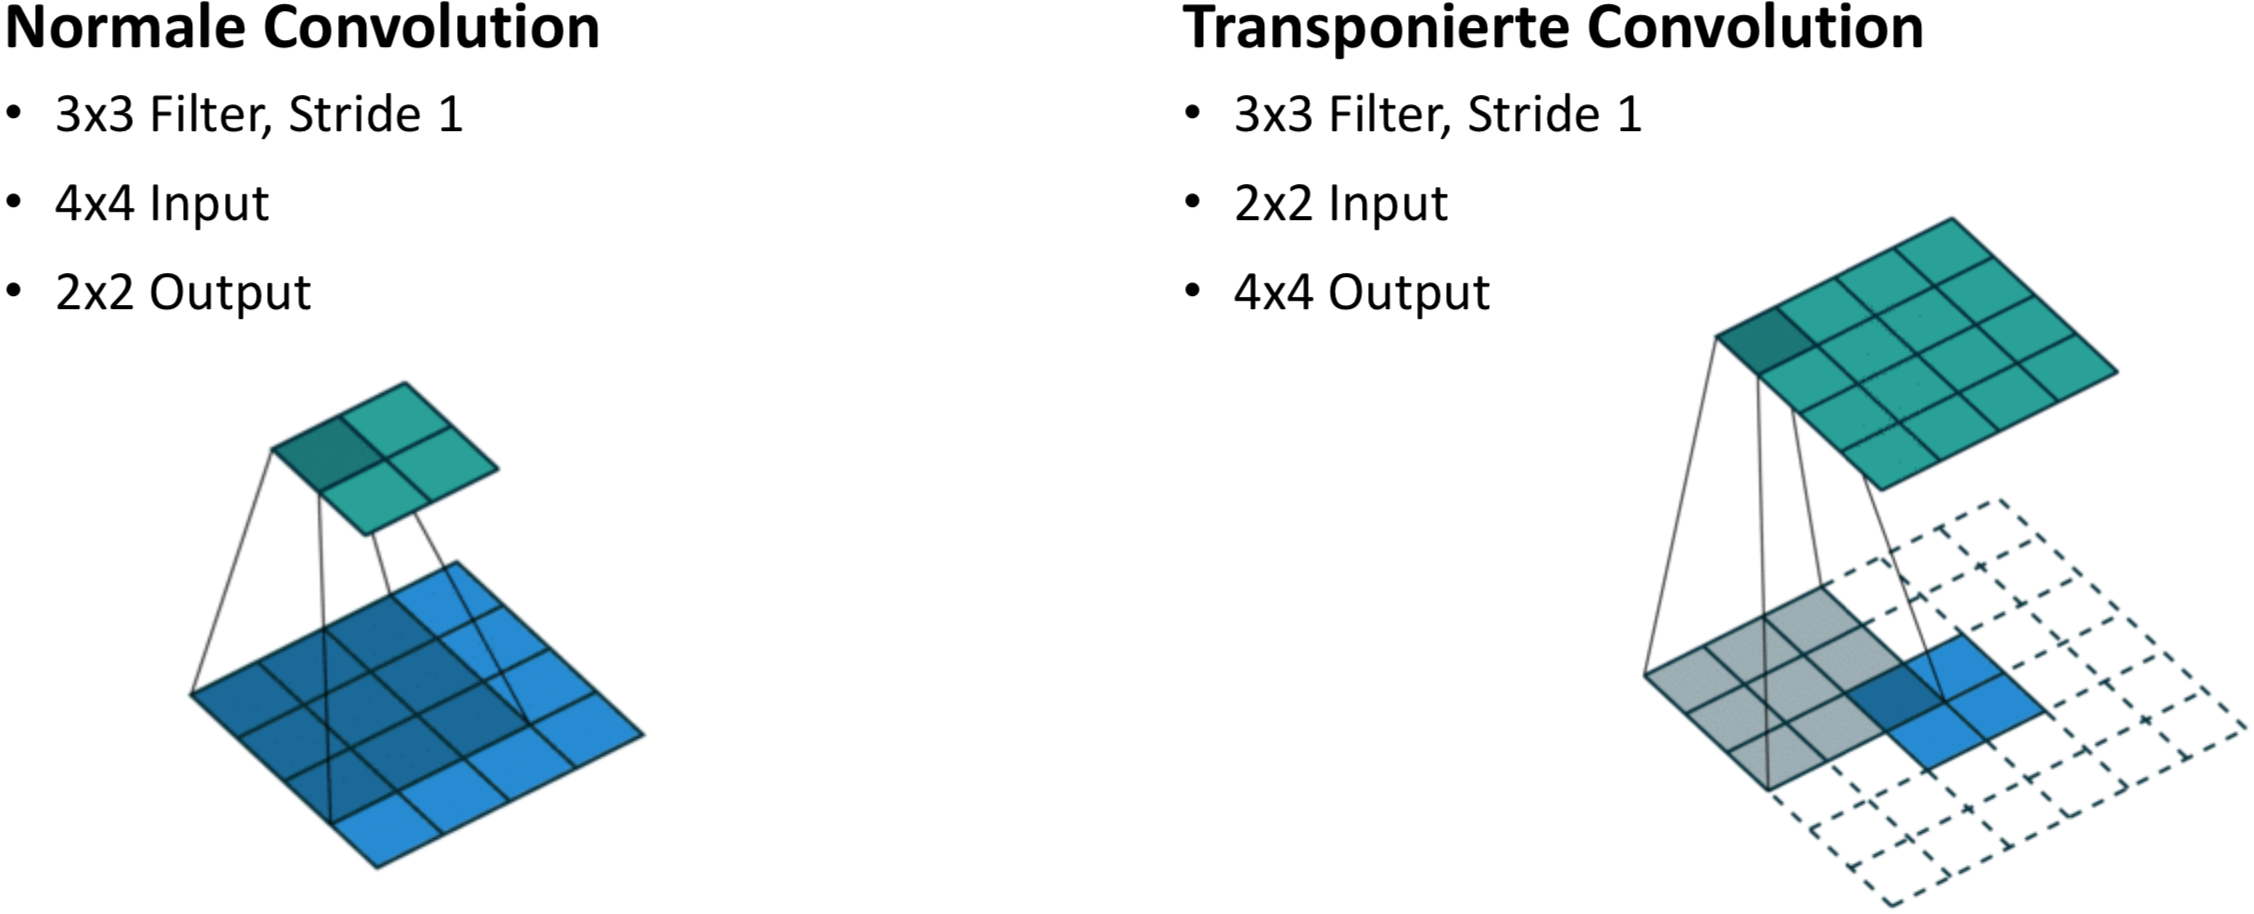
\includegraphics[width=\linewidth]{figures/transposed-convolution.png}\\
	\textbf{Unpooling} Umkehren des Poolings analog zum Backward-Pass (z.B. bei Max-Pooling bekommt das ursprüngliche Maximum alles). Kann nur mit einer Pooling-Schicht verwendet werden, die umgekehrt werden soll $\rightarrow$ Alternative zum Upsampling
	\subsection{Objekterkennung}
	\textbf{Single Shot Detector} Definiere Standard Bounding Boxes (BB) im Bild. Netwerk soll Klasse und Abweichung von einer Standard BB angeben.
	$$L = \frac{1}{N} (L_{conf} + \alpha L_{loc})$$
	mit $L_{conf}$ als Cross-Entropy über die Klassen und $L_{loc} = - \sum_n^N smooth_{l_1}(l_n - g_n)$\\
	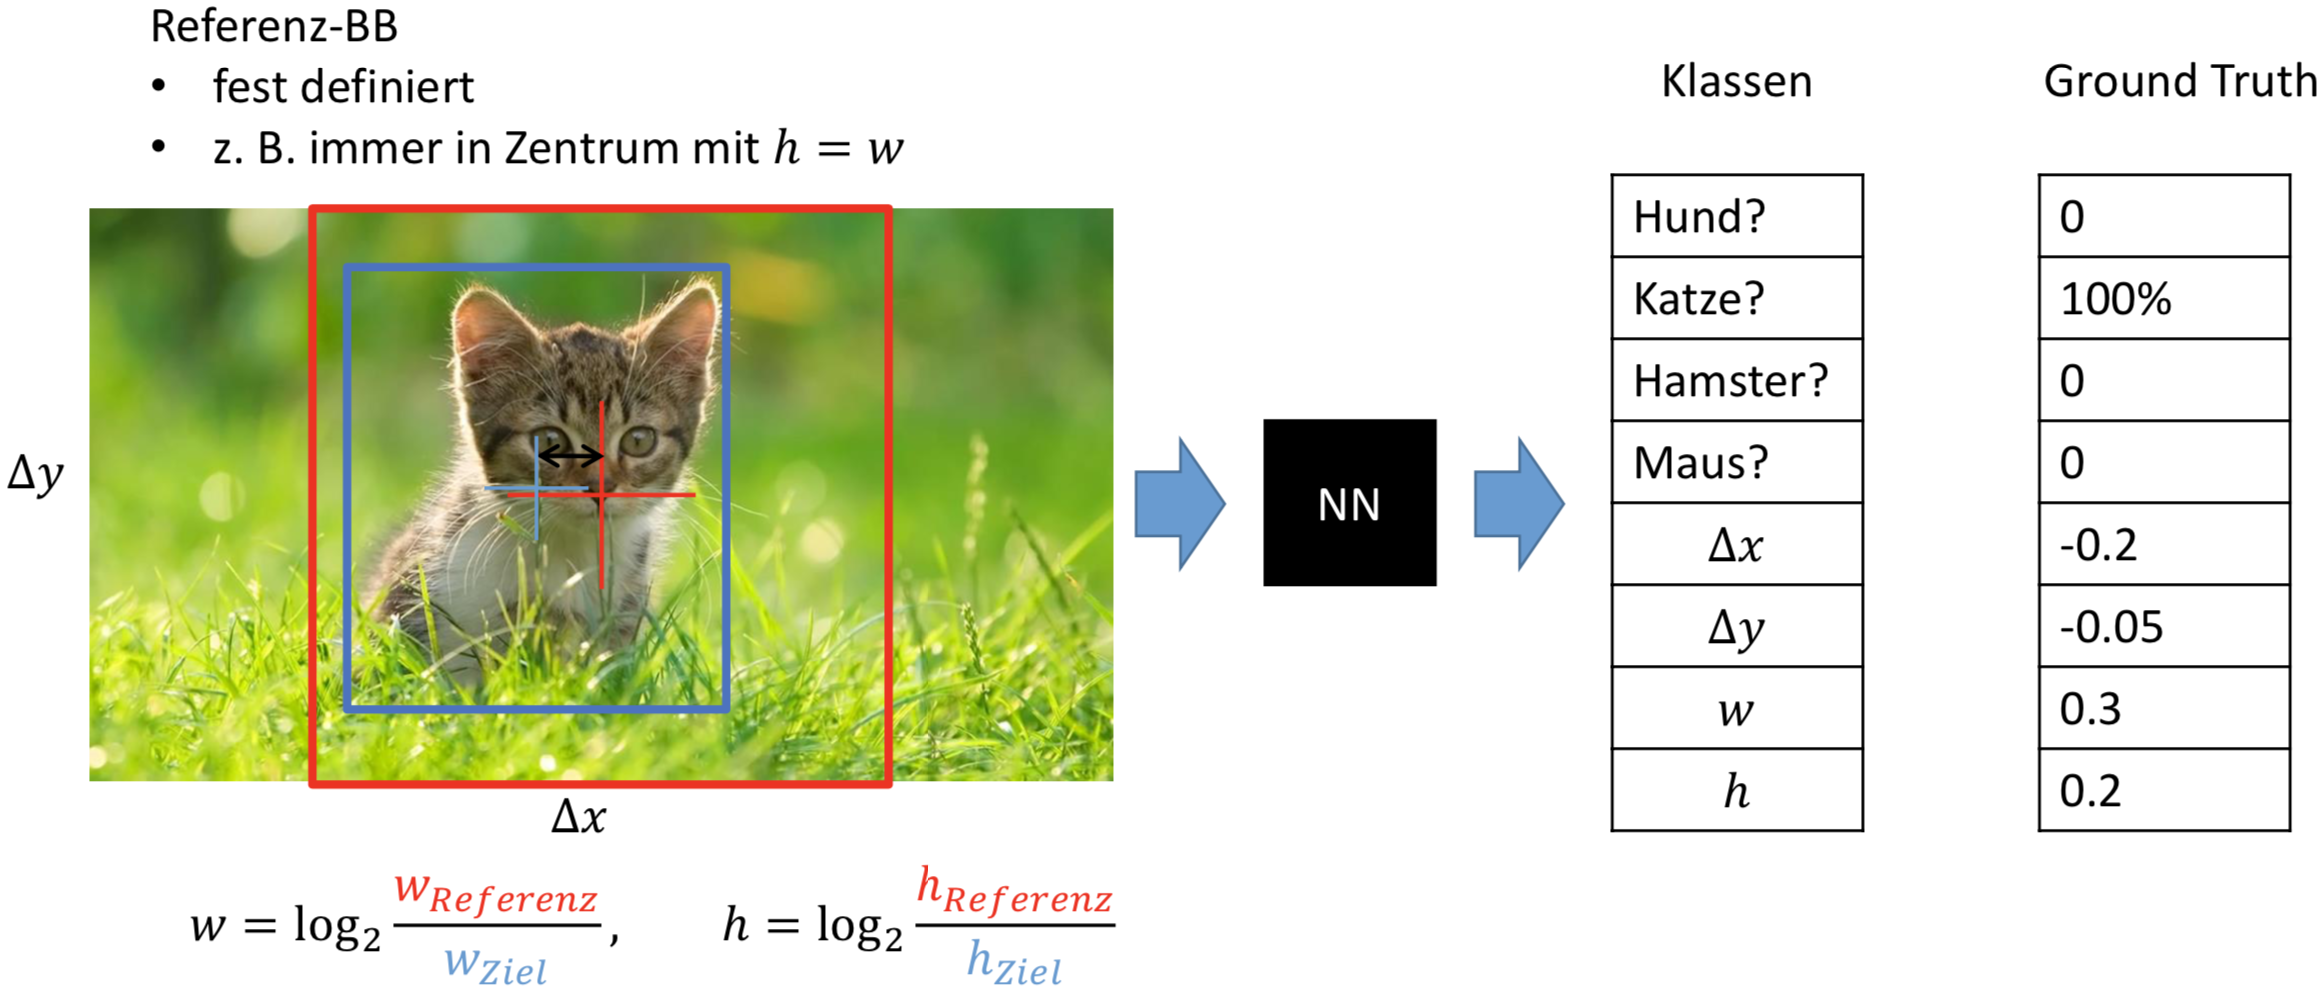
\includegraphics[width=\linewidth]{figures/single-shot-detector.png}\\
	\textbf{Multi Object Detection} mehrere BBs (ca. 4) pro Pixel. BB gilt als gematched, wenn Flächeninhalt der Vorhersage mit BB zu z.B. 50 Prozent übereinstimmt.\\
	\textbf{Non-Maximum Suppression} Da oft mehrere BBs matchen, suche BB mit höchster Konfidenz und lösche alle BBs, die z.B. mind. 50 Prozent Overlapping haben. Wiederhole, bis keine BBs mehr gelöscht wurden.

	\section{Sequence2Sequence}
	Abbildung von Sequenzen auf Sequenzen, z.B. bei OCR (Eingabe: Pixelspalten, Ausgabe: Buchstabenklassifikation) oder Spracherkennung. Kann z.B. mit LSTMs umgesetzt werden.\\
	\textbf{Greedy-Decoder} Ermittelt Klasse durch Maximum auf Ausgabe $\rightarrow$ Entfernen doppelter Zeichen $\rightarrow$ Blanks entfernen\\
	\textbf{Labellings} Beschreibt die Abbilung der Netzausgabe auf sinnvolle Sequenz.
	$$B: L'^{T} \rightarrow L^{\leq T}$$
	$$B(a-ab-) = B(-aa--aabb) = aab$$
	$$B^{-1}(aab) = {a-ab-, ..., aa-ab, ...}$$
	Summiere die Wahrscheinlichkeiten aller möglichen Pfade, die zum gewünschten Label führen.\\
	\textbf{CTC-Loss (Connectionist Temporal Classification)}\\
	Wird angewendet, wenn die Eingabe eine Zeitsequenz der Länge $T$ ist und als Ausgabe eine unalignierte Labelsequenz der Länge $\leq T$ vorliegt\\
	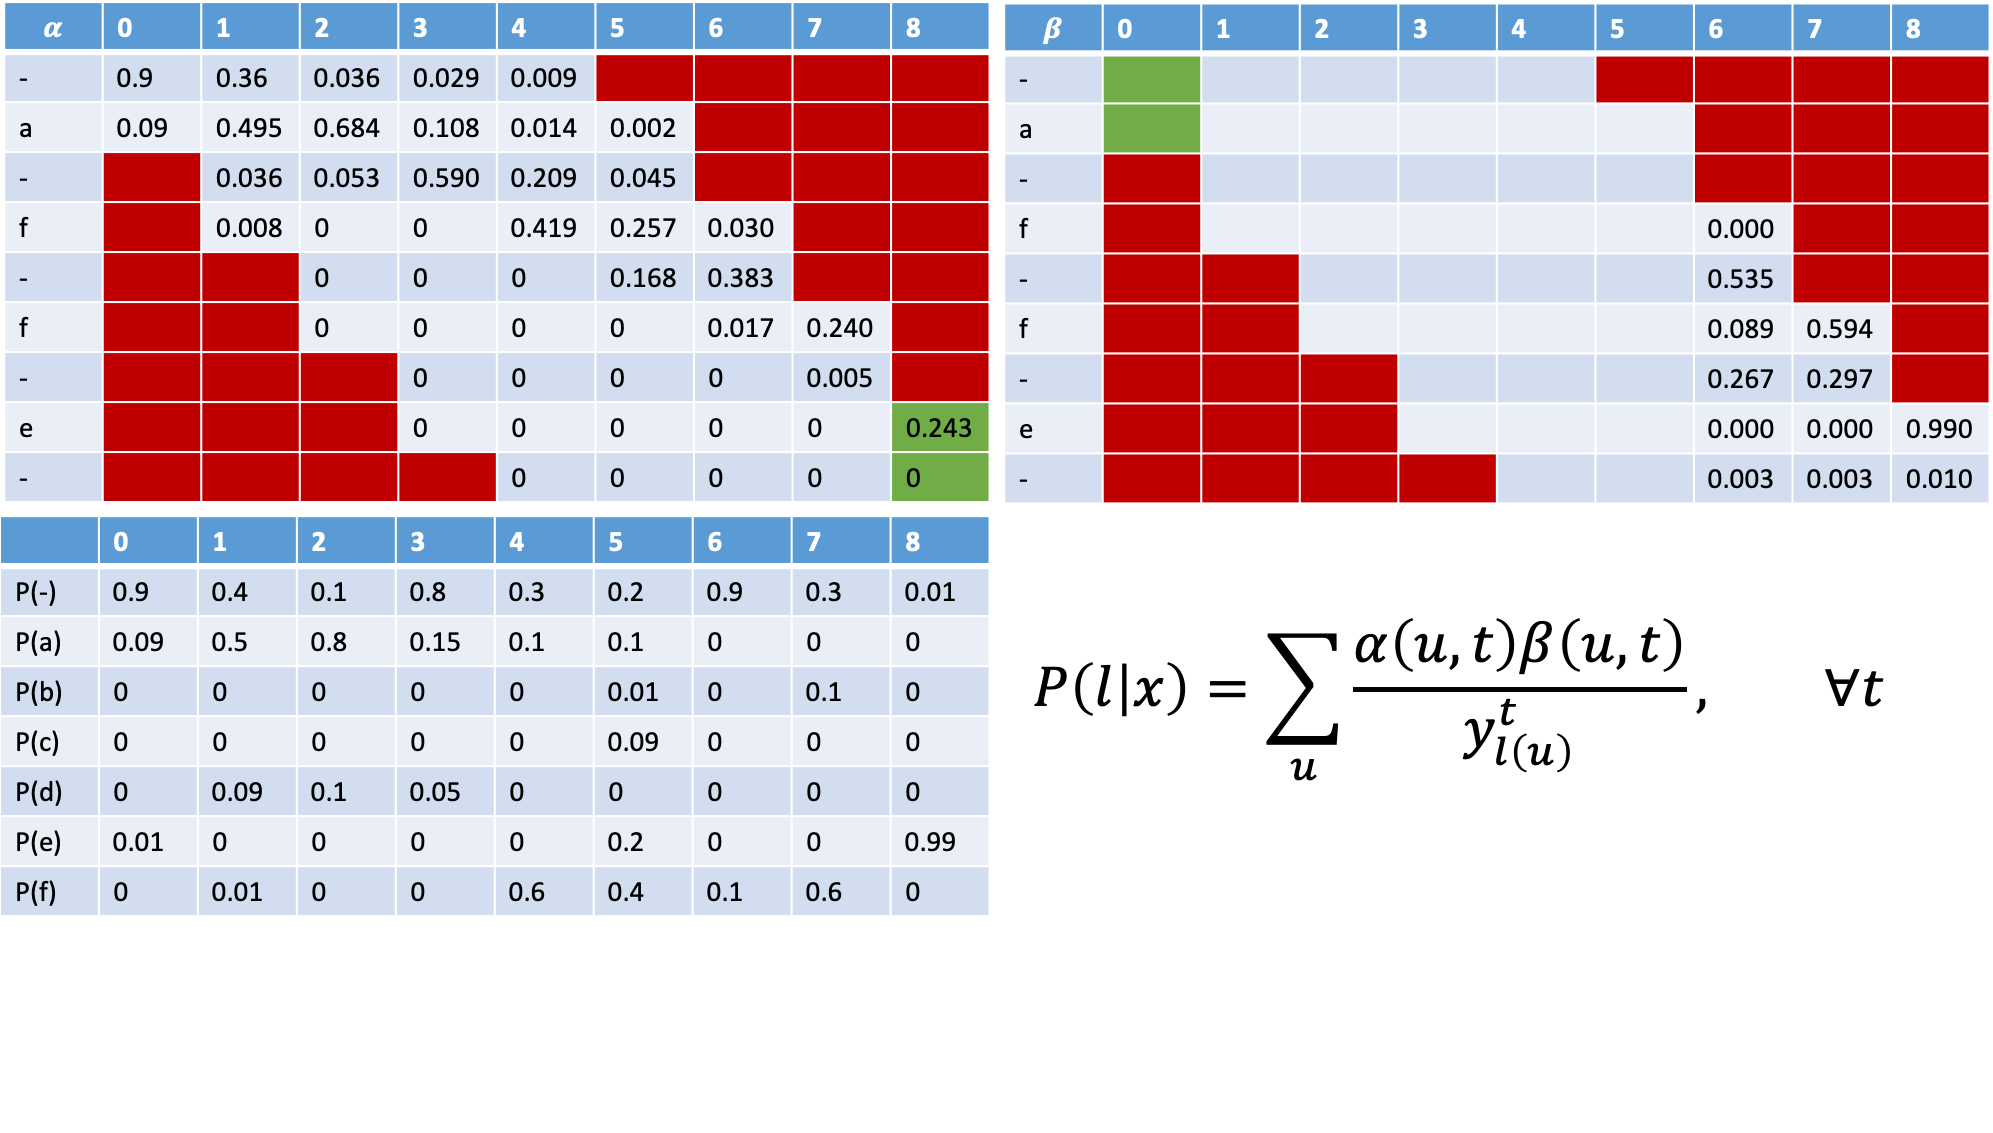
\includegraphics[width=\linewidth]{figures/ctc-algorithmus.png}
	$$P(l|x) = \sum_{\pi \in B^{-1}(l)} P(\pi|x)$$
	mit $l$ als gewünschte Sequenz und $x$ als Netzausgabe\\
	\textit{Loss}: Maximiere $P(l|x)$ bzw. minimiere $-\log(P(l|x))$\\	
\end{document}
